\documentclass[12pt]{article}
\usepackage[backend=biber,natbib=true,style=alphabetic,maxbibnames=10]{biblatex}
\usepackage[utf8]{vietnam}
\addbibresource{/home/nqbh/reference/bib.bib}
\usepackage{tocloft}
\renewcommand{\cftsecleader}{\cftdotfill{\cftdotsep}}
\usepackage[colorlinks=true,linkcolor=blue,urlcolor=red,citecolor=magenta]{hyperref}
\usepackage{amsmath,amssymb,amsthm,float,graphicx,mathtools}
\allowdisplaybreaks
\newtheorem{assumption}{Assumption}
\newtheorem{conjecture}{Conjecture}
\newtheorem{corollary}{Corollary}
\newtheorem{definition}{Definition}
\newtheorem{example}{Example}
\newtheorem{hypothesis}{Hypothesis}
\newtheorem{lemma}{Lemma}
\newtheorem{notation}{Notation}
\newtheorem{note}{Note}
\newtheorem{principle}{Principle}
\newtheorem{problem}{Problem}
\newtheorem{proposition}{Proposition}
\newtheorem{question}{Question}
\newtheorem{remark}{Remark}
\newtheorem{Rule}{Rule}
\newtheorem{theorem}{Theorem}
\usepackage[margin=2cm]{geometry}

\title{Some Thoughts On Learning, Teaching, {\it\&} Research\\Vài Suy Nghĩ Về Việc Học, Việc Dạy, {\it\&} Nghề Nghiên Cứu}
\author{Nguyễn Quản Bá Hồng\footnote{E-mail: {\tt nguyenquanbahong@gmail.com}. Bến Tre City, Việt Nam.}}
\date{\today}

\begin{document}
\maketitle
\begin{abstract}
	This note consists of some pieces of my writing, which are able to be shared and I am willing to share, in order to sharpen my flow of thoughts, to balance my scientific work via various aesthetic forms, \& to track psychologically and mentally my transitions from boyhood to manhood if there is any.
\end{abstract}
\setcounter{secnumdepth}{4}
\setcounter{tocdepth}{3}
\tableofcontents

%------------------------------------------------------------------------------%

\section{An Initial Configuration}

\subsection{Rules}
Mỗi người $P$ (abbr., person) có một xuất phát điểm $\{P(t)\}_{0\le t\le t_0}$ khác nhau, được hưởng hoặc bị ép nhồi các nền tảng giáo dục khác nhau, sự tương tác với những người khác nhau, cùng vô vàn những chuyện \& những biến cố họ gặp trong suốt 1 cuộc đời hoàn toàn khác nhau, thành ra nền tảng nhận thức \& xu hướng phát triển nhận thức, cùng sự hình thành các cấu trúc niềm tin \& các hệ giá trị cơ bản cùng thế giới quan của mỗi người hoàn toàn khác nhau.

Quy tắc đầu tiên ở đây là không phán xét, công kích (e.g., dí trên mạng xã hội) bất cứ ai. Cũng không áp đặt ai, thậm chí cả việc áp đặt ai đó không được áp đặt người khác. Tạo cho người khác 1 cảm giác thoải mái tối thiểu khi tiếp xúc.

Quy tắc thứ 2 là không quá tò mò vào cuộc sống cá nhân của người khác, e.g., stalk in social media -- rình mò trên các nền tảng mạng xã hội, xâm phạm tài khoản  riêng tư cá nhân bất hợp pháp. Keep healthy boundaries for both.

\begin{Rule}[Reset]
	Một phản tư xa hơn trong tương lai có lẽ là chẳng có hành trình phát triển tự thân nào mà đủ sức chống chọi 1 cách hiệu quả với các tương tác xã hội cả, đặc biệt là các tương tác xấu \& các mối quan hệ độc hại (toxic relationships) cả. Khi đó thì tất cả các ghi chú ở đây sẽ bị xóa. Mọi thứ trở về cấu hình sống nhiều mặt để che giấu bản thân phổ dụng.
\end{Rule} 

\subsection{Goals}
This writing activity is one of many ways, which is likely to become the main one, to balance between my scientific work \& personal life. I believe some art will be the tool.

Việc viết lách, theo mình nghĩ, bằng cách này hay cách khác, một lúc nào đó \& theo 1 cách tự nhiên nào đó, cũng sẽ tìm tới những kẻ thích suy nghĩ, những kẻ hay nghĩ nhiều, \& những kẻ mệt mỏi vì cái tật đó, e.g., nhà nghiên cứu, nghiên cứu sinh, các học giả, nói chung là những người làm trong mảng học thuật hoặc phải tiếp xúc nhiều với chữ. Tật hay tài thì chưa biết nhưng ắt hẳn việc viết dùng để sắp xếp mọi thứ trong đầu cho ngăn nắp thì không thể tránh khỏi đối với những người làm việc đầu óc nhiều.

%------------------------------------------------------------------------------%

\section{On Learning -- Bàn Về Việc Học}

%------------------------------------------------------------------------------%

\section{On Teaching -- Bàn Về Việc Dạy}
Tôi gặp Hồng [nam, 27 tuổi] đang loay hoay viết về buổi trò chuyện của hắn với các thầy cô giáo cũ dưới quê.

\begin{quote}
	{\sc Hồng}[28]: Anh định viết thế nào?
	
	{\sc Hồng}[27]: Khó. Chả dễ. Viết lung tung cho đủ ý thì dễ, mà cho hay, cho trơn tru, đọc bắt tai thì khó quá xá.
	
	{\sc Hồng}[28]: Nếu dạng trò chuyện, tâm sự thì anh có thể tham khảo phong cách đối thoại trong 2 cuốn sách \textit{Dám Bị Ghét} \cite{Ichiro_Fumitake2022a} \& \textit{Dám Hạnh Phúc} \cite{Ichiro_Fumitake2022b} của 2 tác giả Nhật Bản \textsc{Kishimi Ichiro \& Koga Fumiake}.
	
	{\sc Hồng}[27]: Nội dung gì nhỉ?
	
	{\sc Hồng}[28]: Bàn về thuyết tâm lý học trường phái Adlerian. Nguyên bản là cuốn \textit{The Science of Living} \cite{Adler2013} của \textsc{Alfred Alder}.
	
	{\sc Hồng}[27]: Để tui đọc thử. Hy vọng không phải mấy cái học thuyết nhảm địt chỉ lý thuyết suông mà không tí thực tế.
\end{quote}

Nghe lời tôi khuyên, hắn bắt đầu viết. Cụ thể như sau.

\subsection{Dạy Trẻ Vùng Quê}
Tui tình cờ trò chuyện với Nhân [nam, 26 tuổi], 1 gia sư dạy các môn Tự nhiên như Toán Lý Hóa Tin, bên cạnh công việc nghiên cứu chưa đâu vào đâu của hắn, ở 1 vùng quê hẻo lánh.
\begin{quote}
	{\sc Hồng}[27]: Thế anh thích dạy? Thích công việc gõ đầu trẻ?
	
	{\sc Nhân}[26]: Cũng không hẳn. Không thích cũng không ghét. Thích vài cái \& cũng ghét 1 đống cái. Ban đầu nghe lời chị nên thử dạy, do công việc nghiên cứu bế tắc, hết đường tiến nên tạm lui về. Bế tắc sao thì sau tui sẽ kể chi tiết. Giờ tập trung vô việc dạy cái đã. Không kể liền có khi mất hồi nào không hay.
	
	Trước tui có về trường cấp 3 cũ để tham gia dạy đội tuyển học sinh giỏi của tỉnh nhà, hồi năm nhất, năm 2 Đại học. Đội tuyển chỉ có 6 đứa, chứ chưa được 8 hay 10 như của mấy tỉnh mạnh như Sài Gòn hay Hà Nội. Mà được cái 6 đứa giỏi, ngoan, chịu làm bài. Tui thích lắm, với hồi trước mấy thầy có phụ tiền cho tui lúc tui bị bệnh nên coi như là báo đáp cái ơn.
	
	Dưới quê thì khác hẳn. Mẹ nó cái vùng không có khỉ để ho mà cò cũng chả thèm gáy. Đa số học sinh không được giỏi cho lắm, toàn mấy dạng báo báo, mà chả dạng báo nào giống dạng báo nào. Những đứa vừa giỏi vừa ngoan, đủ trình để tui dạy hết sức, chắc hiếm như đếm số ngón tay của 1 đứa bị cùi.
	
	{\sc Hồng}[27]: Anh cứ bình tĩnh, việc gì phải xỉ vả thế?
	
	
	
	Tùy vào dạy ai, dạy cái gì, \& dạy ở mức độ nào.
	
\end{quote}


%------------------------------------------------------------------------------%

\section{On Research -- Bàn Về Nghiên Cứu}
It is kind of funny, ironic, and sarcastic that the author of this writing is a dropout PhD student from one of the best research institutes of applied mathematics in Germany.



Khi phải đối đầu với những thứ thật sự khó nhằn, hoàn toàn nằm ngoài hiểu biết hiện tại của 1 cá nhân, thì 1 cách khá đơn giản là bám víu vào những thứ đã biết rõ, dù có thể lặp đi lặp lại 1 cách đơn điệu \& nhàm chán, nhưng lại có trật tự để cân bằng với hỗn loạn -- tượng trưng cho những điều chưa biết \cite{Peterson2018,Peterson2022a,Peterson2022b}.

\begin{example}
	Dạy học bậc phổ thông trở xuống thì ``nhàn'', theo nghĩa là không cần phải nạp quá nhiều kiến thức mới, nhưng phải chú trọng về phương pháp dạy \& truyền đạt kiến thức 1 cách hiệu quả tới các học sinh. Nếu học sinh giỏi, tiếp thu nhanh thì khỏe. Gặp học sinh dốt hoặc đầu gấu thì mệt, đâm ra chán chường, cảm thấy phí phạm thời gian \& nguồn sức lực hạn chế của bản thân.
	
	Nghiên cứu thì lại khác. Trách nhiệm của nghiên cứu là phải đọc thật nhiều, nạp thật nhiều kiến thức để trau dồi bản thân mỗi ngày.***
\end{example}
[...]

Tạm phân loại học giả, theo ý cá nhân (sẽ bổ sung thêm):
\begin{itemize}
	\item Học giả làm các mảng, lĩnh vực năng động, với năng suất xuất bản ấn phẩm khoa học cao, thường được trích dẫn nhiều nhờ sự năng động của cộng đồng khoa học tương ứng.
	\item Học giả làm các mảng khó nhằn, trừu tượng, nên tần suất xuất bản ấn phẩm khoa học khá thấp, nhưng các bài này đều ở dạng nặng đô (hardcore), thường ít được trích dẫn vì kén độc giả. Nếu bài báo đó trở thành cornerstone thì lại được trích dẫn nhiều đến rất nhiều, na ná dạng benchmark cases for industrial purposes của loại 1 (data mẫu chuẩn để các người làm nghiên cứu R\&D ở các lĩnh vực công nghiệp dùng).
\end{itemize}
Ưu điểm của loại 1 là đi hội nghị thường xuyên. Mà đa số mấy hội nghị này giàu do dính đến công nghiệp hoặc dịch vụ số hóa (AI{\tt/}DL{\tt/}ML) nên chắc đồ ăn nhiều \& ngon, ít nhất cũng ăn đứt mấy bữa tiệc giản đơn gồm trà, cafe máy cùng vài cái bánh quy như các hội nghị toán lý thuyết ở Pháp mà hồi mình học Master (hay chỉ có mấy chỗ nằm ở rìa của Pháp là vậy nhỉ?). Mà thực ra lúc mấy giáo sư Toán thảo luận với nhau, thay vì nhắm nháp cafe \& ăn bánh quy, vài người lại say xưa thảo luận mà ăn (nhầm?) phấn trắng.

Chắc mình thuộc loại 2, hoặc ít nhất là mình tự ép bản thân thuộc loại 2 (nên gọi là \textit{giả học -- fake scholar} thì hợp hơn). Trong khi loại 1 thì tạo cảm giác năng động, tràn trề của sức trẻ, thì loại 2 hoàn toàn ngược lại, mà phần lớn là phải cày background khá nhiều \& nặng, \& 1 trong những cái mệt nhất nhưng rewarding nhất của loại 2 là làm các công trình khoa học liên ngành, kết nối các kết quả mạnh nhất của các lĩnh vực lý thuyết với nhau.

Có 1 bài viết phân loại học giả hay của GS. Nguyễn Tiến Zũng của ĐH Toulouse. Tiếc là sau khi GS Zũng hỗn chiến với bác  Phùng Xuân Nhạ thì website cá nhân \url{http://zung.zetamu.net/} của GS trước bị lỗi font \& giờ có lẽ đã bay màu.

\subsection{Trends \& Choices -- Các Xu Hướng \& Lựa Chọn}	

\begin{quote}
	{\sc Nhân}[23]: Thế anh có biết những sở thích thời học sinh của 1 người ảnh hưởng thế nào đến xu hướng các lựa chọn chuyên ngành trong tương lai của họ không?
	
	{\sc Hồng}[28]: Tôi không rõ lắm. Cụ thể sao?
	
	{\sc Nhân}[23]: Tui sẽ lấy ví dụ về ngành Toán. Vì nó là cái duy nhất tui rành, ít hơn là rành hơn ối thứ còn lại.
	
	Những học sinh thích giải phương trình, hệ phương trình ở Toán Sơ Cấp nhưng không thích Tin học thường sẽ có xu hướng chọn các ngành lý thuyết trừu tượng, như Đại Số, Hình Học Đại Số. 
	
	Những người thích bất đẳng thức ở Toán Sơ Cấp thường sẽ có xu hướng chọn hướng Giải tích, đặc biệt là hướng Phương Trình Vi Phân Đạo Hàm Riêng (Partial Differential Equations, abbr., PDEs) vì hướng này chủ yếu đánh giá (estimation), chặn (bound), i.e., các bất đẳng thức giữa các không gian hàm. Như vậy, xu hướng thích đánh giá các đại lượng liên quan tới các hàm sơ cấp ở Toán Sơ Cấp thường sẽ phát triển thành niềm đam mê việc đánh giá các đại lượng liên quan đến hàm hoặc các đối tượng toán học trừu tượng hơn.

	1 câu hỏi điển hình của các nhà Giải tích học (mathematical analysts) khi thảo luận các vấn đề toán học liên quan đến PDEs là:
	
	- \textit{Do you think it is smooth (or regular) enough? -- Anh nghĩ nó có đủ trơn (hay nhớt) không?}
	
	- \textit{It seems a little rough at the initial phase. But it will be smoother later. Oh, now it's already smooth enough for us. Let's do{\tt/}play with it. -- Nhìn có vẻ hơi thô trong giai đoạn đầu (màn dạo đầu?). Nhưng rồi nó sẽ trơn hơn thôi. Ồ nhìn này, nó đủ trơn rồi kìa. Nào, chúng ta cùng xử{\tt/}quất{\tt/}chơi nó (vấn đề giải tích này) thôi}.
	
	Hàm đối tượng trơn chưa đủ, để đặt tốt 1 bài toán, miền xác định, i.e., nơi hàm đó sống, phải đủ trơn nữa, tức là cái mép (boundary $\Gamma\coloneqq\partial\Omega$) của cái miền $\Omega$ phải đủ trơn để xài các công thức tích phân từng phần (integration by parts formulas or Green's identities) để tạo ra dạng yếu (weak formulation or variational formulation). Những miền quá thô, e.g., có các góc nhọn (rough boundaries with corners), kỳ dị (singularities), chỗ nhọn dễ bị đâm (cusps), có nhiều lỗ (holes) hoặc gai (thorns) sẽ không thích hợp để làm chỗ chơi đối với các nghiệm trơn, dẫu mấy cái nghiệm đó có trơn chùi cỡ nào đi chăng nữa, vẫn không đảm bảo an toàn để chơi với chúng. Safety 1st.
	
	Ngoài lề, dù hay thắc mắc với việc đòi hỏi các nghiệm trơn, nghiệm nhớt của phương trình vi phân đạo hàm riêng có đủ trơn, đủ nhớt hay không để mà có thể vô tư chơi với chúng, tuổi thơ của các nhà giải tích cho thấy họ không có liên quan đến bất kỳ về tình dục sớm kiểu con nít quỷ hoặc sống thử, hay lạm dụng tình dục nào cả. Cho nên việc đề xuất những khẳng định kiểu như của {\sc Sigmund Freud}, e.g., các nhà toán học loay hoay với câu hỏi đủ trơn thường có tuổi thơ liên quan đến các vấn đề tình dục sớm do cha mẹ hoặc người tình của họ không quan hệ kín đáo để cho con cái vô tình bắt gặp hoặc các sang chấn tâm lý do chịu lạm dụng tình dục từ sớm; hoặc lý luận kiểu {\sc Malcolm Gladwell} trong quyển \textit{Outliers: The Story of Success} \cite{Gladwell2008} hay bản dịch \textit{Những Kẻ Xuất Chúng: Cái Nhìn Mới Lạ Về Nguồn Gốc Của Thành Công} \cite{Gladwell_outlier} ngụ ý việc tiếp xúc 1 cách vô thức với các từ gợi hình (gợi dục) tác động đến tiềm thức sâu bên dưới ý thức dẫn đến xu hướng chỉ thích làm với các đối tượng đủ trơn hoặc cuồng với các khái niệm đủ nhớt, etc. là hoàn toàn không có sơ sở.
	
	{\sc Hồng}[28]: What is so wrong with you?
\end{quote}

\subsection{Signs -- Các Dấu Hiệu}

\subsubsection{Personal systems of notations, abbreviations, \& conventions}
Bộ (tuple), tập hợp (set), hay hệ thống ký hiệu, viết tắt, quy ước cá nhân -- a personal set{\tt/}system of notations, abbreviations, \& conventions -- của 1 nhà khoa học tự nhiên thiên về lý thuyết hơn là về tính toán engineering thuần ứng dụng, e.g., nhà toán học (mathematicians), nhà vật lý (physicists), nhà khoa học máy tính (computer scientist), etc. là dấu hiệu đầu tiên cho biết trình độ của họ. Đơn giản vì các môn khoa học này có 1 đặc thù là đòi hỏi độ nhất quán (consistency) cực kỳ cao cho nên 1 hệ thống ký hiệu nhất quán, không mâu thuẫn, tiện dụng, không tạo ra bất kỳ sự mơ hồ, mờ mập (confusion) sẽ phản ánh phần nào trình độ của họ. Đấy là dấu hiệu dễ nhận biết đầu tiên -- nhưng còn xa so với mức phán xét -- của 1 người làm khoa học giỏi hoặc ít nhất là có 1 người thầy, người hướng dẫn giỏi.

Riêng các nhà hóa học (chemists) thì có lẽ họ được quy định chung bởi các danh pháp quốc tế như International Union of Pure and Applied Chemistry (abbr., IUPAC)\footnote{\url{https://en.wikipedia.org/wiki/International_Union_of_Pure_and_Applied_Chemistry}.} nên không{\tt/}chưa thể dùng hệ thống ký hiệu cá nhân để đánh giá sơ bộ. Có lẽ mình nên kết thêm vài đứa bạn chuyên ngành Hóa để hiểu thêm (vừa đủ).

Thus, a good advice for young science students: Build, polish, and perfect endlessly your personal system of notations and conventions so well that it will fit perfectly to any of, or at least most of, your research fields. Then you can effortlessly attack each of them, connect them, play with the interaction between them and beyond, and even foresee the hidden structure in the realm of abstractness.

Lời khuyên (tự thân) này na ná câu trích dẫn sau của Abraham Lincoln về việc đầu tư khâu chuẩn bị kỹ lưỡng:
\begin{quote}\it
	``Give me 6 hours to chop down a tree and I will spend the 1st 4 sharpening the axe.'' -- {\sc Abraham Lincoln} (1809--1865) -- 16th President of the United States (1861--1865)
\end{quote}

\subsubsection{Consistency -- Sự nhất quán}

\begin{question}
	Liệu có nên (dấn thân) theo 1 nghề cố định, không chịu{\tt/}thèm nhảy nghề không? 
\end{question}
Hiển nhiên 1 câu hỏi khó muôn thở. Khó chịu lẫn khó nhằn theo nhiều nghĩa. Nghĩa thứ nhất là nó không rõ ràng, \& sự không rõ ràng đến từ việc bản thân nó phụ thuộc vào quá nhiều yếu tố không thể xác định hết như các yếu tố về phương diện vật chất, e.g., lương, tài chính; cũng như các yếu tố về phương diện tinh thần, e.g., ý nghĩa công việc, cân bằng công việc--cuộc sống (work-life balance), sự phát triển cá nhân, cùng sự tương tác lẫn nhau giữa các yếu tố trong 2 phương diện đó; \& nếu lùi xa hơn nữa về quá khứ thì chúng cũng phụ thuộc vào nhiều yếu tố ban đầu của 1 cá nhân như điểm xuất phát mà bố mẹ mang lại, hoàn cảnh như khả năng tài chính của gia đình, sự ủng hộ từ dòng họ, \& ảnh hưởng của các mâu thuẫn, lục đục nội bộ trong 2 môi trường nền tảng dđó.

Tôi không hề nghĩ sẽ cố trả lời 1 cách hoàn hảo câu hỏi này hay giải quyết vấn đề này. Đồng ý là tôi ngu, nhưng chưa ngu đến mức vậy. Chưa kể có bất kỳ câu trả lời nào không (no guarantee of existence), nếu có thì cũng không hề có câu trả lời duy nhất (even if the existence is assumed, the nonuniqueness is still valid), cũng như chưa \& sẽ không chả có câu trả lời nào sẽ thỏa mãn hết tất cả các phương diện giá trị được suy xét ở \textit{biểu diễn phân hoạch các giá trị \& ý nghĩa của cuộc đời} (\textit{a decomposition of values \& meanings in life}) sẽ được xét đến trong Sect. \ref{sect: bullshit theory on live}: \textit{A Bullshit Theory on How To Live -- 1 Lý Thuyết Nhảm Nhí Về Cách Sống}.

\begin{figure}[H]
	\centering
	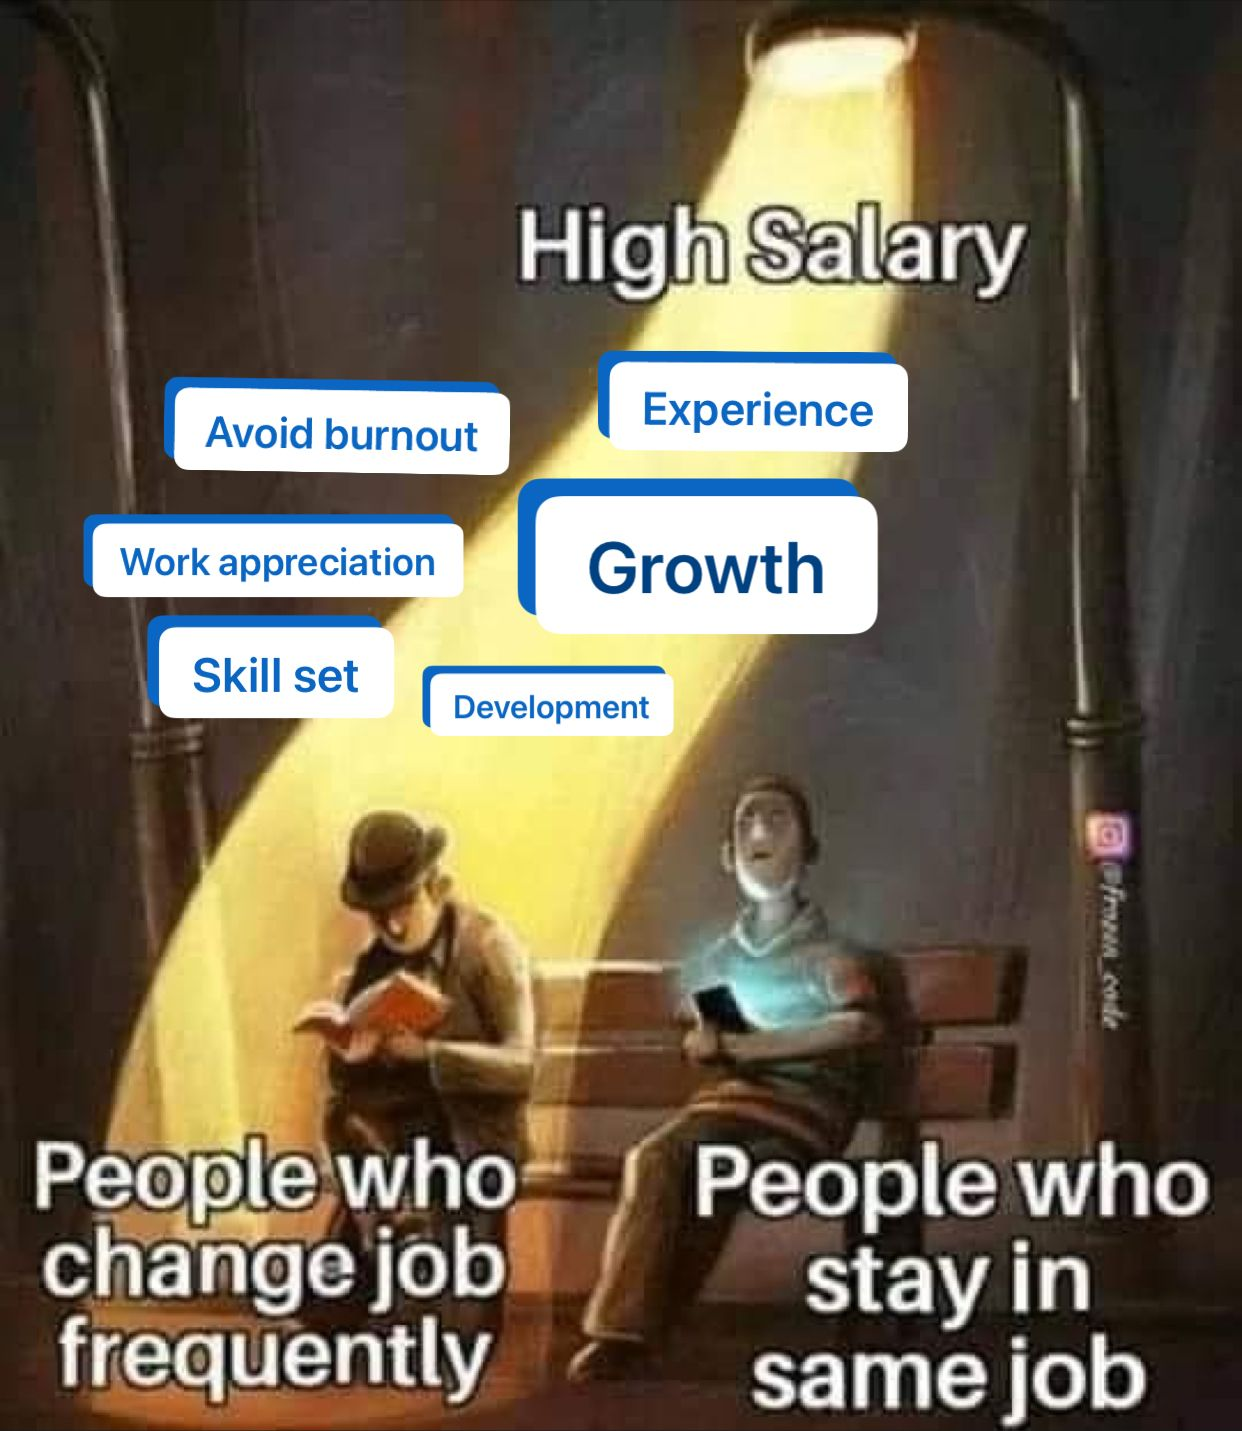
\includegraphics[scale=.15]{high_salary}
	\caption{Credit: \href{https://www.linkedin.com/posts/judy-soloai_i-didnt-learn-this-in-school-i-learned-activity-7089014937494179840-jTze/}{Linkedin{\tt/}Judy Soloai{\tt/}I didn't learn this in school}.}
\end{figure}

\subsubsection{Accuracy -- Tính chính xác}

\subsubsection{Simplicity -- Sự giản đơn}

\subsubsection{Minimality -- Sự tối giản}
\cite{Chi2022}.

\subsubsection{Vigor -- Khí lực, sức mãnh liệt}

\subsubsection{Rigour -- Tính chặt chẽ}

\subsubsection{Visionary -- Nhìn Xa Trông Rộng}

%------------------------------------------------------------------------------%

\section{A Bullshit Theory on How To Live -- 1 Lý Thuyết Nhảm Nhí Về Cách Sống}
\label{sect: bullshit theory on live}
Maps of Meanings.

\section{Miscellaneous}

%------------------------------------------------------------------------------%

\appendix

%------------------------------------------------------------------------------%

\printbibliography[heading=bibintoc]
	
\end{document}